\documentclass[border=8pt]{standalone}
\usepackage{amsmath,amssymb,bm}
\usepackage{xcolor}
\usepackage{tikz}
% --- deck palette (meson purple, same values as the previous tables) ---
\definecolor{P}{HTML}{4B1D8F}
\definecolor{band}{HTML}{F3E8FA}
\definecolor{lcol}{HTML}{E7D6F5}
\definecolor{rule}{HTML}{CDB7E6}
\definecolor{G}{HTML}{6F6585}

\begin{document}
\large
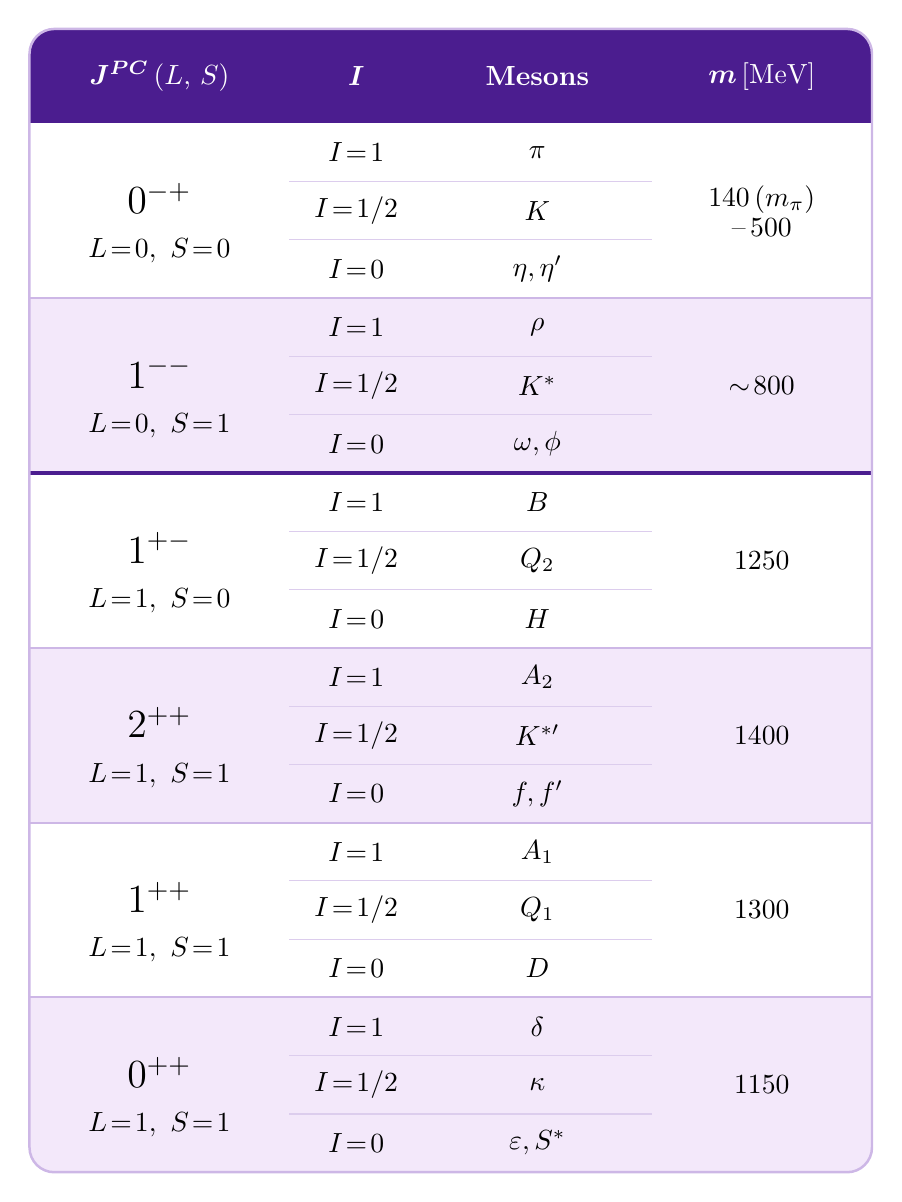
\begin{tikzpicture}
  \begin{scope}
    \clip[rounded corners=9pt] (0,0) rectangle (10.7,-14.52);
    \fill[P] (0,0) rectangle (10.7,-1.2);
    \fill[band] (0,-3.42) rectangle (10.7,-5.64);
    \fill[band] (0,-7.86) rectangle (10.7,-10.08);
    \fill[band] (0,-12.299999999999999) rectangle (10.7,-14.52);
  \end{scope}
  % thin separators between the isospin sub-rows, strong ones between multiplets
  \draw[rule!70,line width=.4pt] (3.3,-1.94) -- (7.9,-1.94);
  \draw[rule!70,line width=.4pt] (3.3,-2.6799999999999997) -- (7.9,-2.6799999999999997);
  \draw[rule!70,line width=.4pt] (3.3,-4.16) -- (7.9,-4.16);
  \draw[rule!70,line width=.4pt] (3.3,-4.9) -- (7.9,-4.9);
  \draw[rule!70,line width=.4pt] (3.3,-6.38) -- (7.9,-6.38);
  \draw[rule!70,line width=.4pt] (3.3,-7.119999999999999) -- (7.9,-7.119999999999999);
  \draw[rule!70,line width=.4pt] (3.3,-8.6) -- (7.9,-8.6);
  \draw[rule!70,line width=.4pt] (3.3,-9.34) -- (7.9,-9.34);
  \draw[rule!70,line width=.4pt] (3.3,-10.819999999999999) -- (7.9,-10.819999999999999);
  \draw[rule!70,line width=.4pt] (3.3,-11.559999999999999) -- (7.9,-11.559999999999999);
  \draw[rule!70,line width=.4pt] (3.3,-13.04) -- (7.9,-13.04);
  \draw[rule!70,line width=.4pt] (3.3,-13.78) -- (7.9,-13.78);
  \draw[rule,line width=.7pt] (0,-3.42) -- (10.7,-3.42);
  \draw[rule,line width=.7pt] (0,-7.86) -- (10.7,-7.86);
  \draw[rule,line width=.7pt] (0,-10.079999999999998) -- (10.7,-10.079999999999998);
  \draw[rule,line width=.7pt] (0,-12.299999999999999) -- (10.7,-12.299999999999999);
  \draw[P,line width=1.3pt] (0,-5.64) -- (10.7,-5.64);   % between L=0 and L=1
  \draw[rule,line width=.9pt,rounded corners=9pt] (0,0) rectangle (10.7,-14.52);
  % header
  \node[text=white] at (1.65,-0.6) {$\bm{J^{PC}}$\,{\normalsize\mdseries($L$, $S$)}};
  \node[text=white] at (4.15,-0.6) {$\bm{I}$};
  \node[text=white] at (6.45,-0.6) {\bfseries Mesons};
  \node[text=white] at (9.3,-0.6) {$\bm{m}$\,{\normalsize\mdseries[MeV]}};
  \node[font=\Large] at (1.65,-2.15) {$0^{-+}$};
  \node[font=\normalsize] at (1.65,-2.8200000000000003) {$L\!=\!0,\ S\!=\!0$};
  \node at (9.3,-2.3099999999999996) {\shortstack{140\,($m_\pi$)\\[-1pt]--\,500}};
  \node at (4.15,-1.5699999999999998) {$I\!=\!1$};
  \node at (6.45,-1.5699999999999998) {$\pi$};
  \node at (4.15,-2.3099999999999996) {$I\!=\!1/2$};
  \node at (6.45,-2.3099999999999996) {$K$};
  \node at (4.15,-3.05) {$I\!=\!0$};
  \node at (6.45,-3.05) {$\eta,\eta'$};
  \node[font=\Large] at (1.65,-4.37) {$1^{--}$};
  \node[font=\normalsize] at (1.65,-5.04) {$L\!=\!0,\ S\!=\!1$};
  \node at (9.3,-4.529999999999999) {$\sim\!800$};
  \node at (4.15,-3.79) {$I\!=\!1$};
  \node at (6.45,-3.79) {$\rho$};
  \node at (4.15,-4.529999999999999) {$I\!=\!1/2$};
  \node at (6.45,-4.529999999999999) {$K^{*}$};
  \node at (4.15,-5.27) {$I\!=\!0$};
  \node at (6.45,-5.27) {$\omega,\phi$};
  \node[font=\Large] at (1.65,-6.59) {$1^{+-}$};
  \node[font=\normalsize] at (1.65,-7.26) {$L\!=\!1,\ S\!=\!0$};
  \node at (9.3,-6.75) {$1250$};
  \node at (4.15,-6.01) {$I\!=\!1$};
  \node at (6.45,-6.01) {$B$};
  \node at (4.15,-6.75) {$I\!=\!1/2$};
  \node at (6.45,-6.75) {$Q_2$};
  \node at (4.15,-7.49) {$I\!=\!0$};
  \node at (6.45,-7.49) {$H$};
  \node[font=\Large] at (1.65,-8.81) {$2^{++}$};
  \node[font=\normalsize] at (1.65,-9.48) {$L\!=\!1,\ S\!=\!1$};
  \node at (9.3,-8.97) {$1400$};
  \node at (4.15,-8.23) {$I\!=\!1$};
  \node at (6.45,-8.23) {$A_2$};
  \node at (4.15,-8.97) {$I\!=\!1/2$};
  \node at (6.45,-8.97) {$K^{*\prime}$};
  \node at (4.15,-9.71) {$I\!=\!0$};
  \node at (6.45,-9.71) {$f,f'$};
  \node[font=\Large] at (1.65,-11.029999999999998) {$1^{++}$};
  \node[font=\normalsize] at (1.65,-11.7) {$L\!=\!1,\ S\!=\!1$};
  \node at (9.3,-11.189999999999998) {$1300$};
  \node at (4.15,-10.449999999999998) {$I\!=\!1$};
  \node at (6.45,-10.449999999999998) {$A_1$};
  \node at (4.15,-11.189999999999998) {$I\!=\!1/2$};
  \node at (6.45,-11.189999999999998) {$Q_1$};
  \node at (4.15,-11.929999999999998) {$I\!=\!0$};
  \node at (6.45,-11.929999999999998) {$D$};
  \node[font=\Large] at (1.65,-13.249999999999998) {$0^{++}$};
  \node[font=\normalsize] at (1.65,-13.919999999999998) {$L\!=\!1,\ S\!=\!1$};
  \node at (9.3,-13.409999999999998) {$1150$};
  \node at (4.15,-12.669999999999998) {$I\!=\!1$};
  \node at (6.45,-12.669999999999998) {$\delta$};
  \node at (4.15,-13.409999999999998) {$I\!=\!1/2$};
  \node at (6.45,-13.409999999999998) {$\kappa$};
  \node at (4.15,-14.149999999999999) {$I\!=\!0$};
  \node at (6.45,-14.149999999999999) {$\varepsilon,S^{*}$};
\end{tikzpicture}
\end{document}
